\chapter{Implementation}
\label{chap:Implementation}
In this chapter we explain the infrastructure that performs all the necessary steps to produce an efficient feedback. A general overview is given and for each section, we describe in particular the tools as well as the way we manipulated the data in order to obtain the information useful for the user. The chapter is divided in two parts: the first part focuses on the back-end and the services we used to extract the features we described in \ref{chap:Speech Recognition}. The second part describe the front-end, that is, the \textit{Android}\footnote{\url{https://www.android.com}} application (called \textbf{PARLA}\footnote{\url{https://github.com/davideberdin/PARLA}}) with a particular focus on the feedback page and the general usage.

\section{General architecture}
\label{sec:general_architecture}

In \ref{fig:general_architecture} is shown the general architecture of the infrastructure.
The flow displays only the \textit{pronunciation testing} phase:

\begin{itemize}
	\item[1)] User says the sentence using the internal microphone of the smartphone (or through the headset)
	\item[2)] The application sends the audio file to the \textit{Speech Recognition service}
	\item[3)] The result of step 2 is sent to the \textit{Gaussian Mixture Model service}
	\item[4)] The result of step 3 is sent back to the application where a \textit{Feedback page} is displayed
	\item[5)] A short explanation for each chart is given to the user
	\item[6)] Back to step 1
\end{itemize}

\noindent The flow described above is the main feature of the whole project. Although, the application supplies other two important functionalities that are described more in detail in \ref{sec:android_app}. The first one is related to \textbf{critical listening} where the user is able to listen to the \textit{Native pronunciation} as well as to its one. This feature have a big impact on improving the pronunciation because it pushes the user to understand the differences as well as to emulate the way native speakers pronounce a specific sequence of words. The second feature regards the \textbf{history} (or progress). This page shows the trend of the user based on all the pronunciation he/she made during the usage of PARLA. The purpose of the history page is to help the user to see the progresses and to get an idea of how to improve the pronunciation. \\

\begin{figure}[!ht]
	\centering
	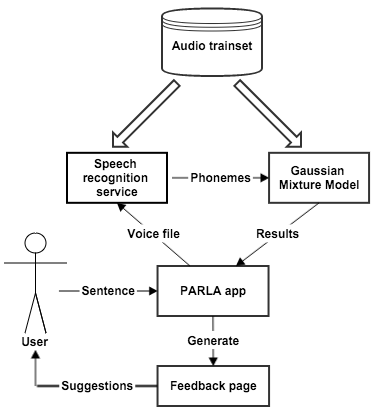
\includegraphics[scale=0.6]{Figures/general_architecture.png}
	\caption{General architecture of the infrastructure}
	\label{fig:general_architecture}
\end{figure}

\subsubsection{Implementation procedure}
\label{ssec:procedure}

Several step were made before to reach the architecture depicted in \ref{fig:general_architecture}. Generally speaking, we divided the implementation in two main categories: the first is composed by the \textit{data collection and training} phase whereas the second is formed by the \textit{mobile application} and \textit{server communication}. \\

\noindent The very first step was to collect the data from native speakers and apply some pre-processing techniques in such way that we were able to obtain only the information we needed to train the two services we had on the server.After the data collection, we trained both the models with the information we extracted in the previous step. The detailed procedures are described in \ref{ssec:training_sr_model} and \ref{ssec:training_gmm}. \\
\noindent When the training phase was completed, we set up the services and used \textit{REST} calls to communicate with the mobile application. These two parts were developed at the same time and are described in detail in \ref{sec:android_app}.


\section{Data collection}
\label{sec:data_collection}

 We recorded 8 people divided  at the University of Rochester using \textit{Audacity}\footnote{\url{http://audacityteam.org}}.

\subsection{Data pre-processing}
\label{ssec:pre_processing}

Data pre-processing subsection

\section{Server}
\label{sec:server}

Here the server description

\begin{figure}[!ht]
	\centering
	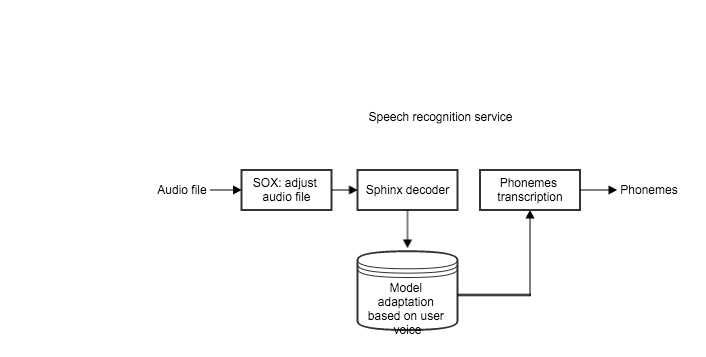
\includegraphics[scale=0.6]{Figures/sphinx_service.png}
	\caption{Architecture of the Speech recognition service}
	\label{fig:sphinx_service}
\end{figure}

\begin{figure}[!ht]
	\centering
	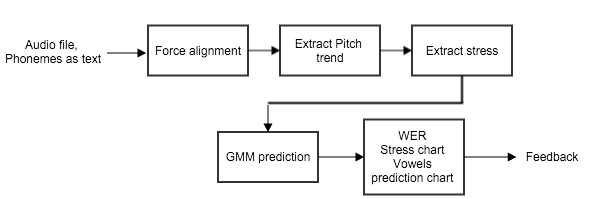
\includegraphics[scale=0.6]{Figures/gmm_service.png}
	\caption{Architecture of the Gaussian Mixture Model service}
	\label{fig:gmm_service}
\end{figure}

\subsection{Training the Speech Recognition model} 
\label{ssec:training_sr_model}

Here the way we trained the speech recognition model

\subsection{Training the Gaussian Mixture Model}
\label{ssec:training_gmm}

Here the way we trained the gmm model \\
BIC, AIC and other things here


%%%%%%%%%%%%%%%%%%%%%%%%%%%%%%%%%%%%%%%%%%%%%%%%%%%%%%%%%%%%%%%%%%%%%%%%%%%%%%%%
%%%%%							ANDROID PART							   %%%%%
%%%%%%%%%%%%%%%%%%%%%%%%%%%%%%%%%%%%%%%%%%%%%%%%%%%%%%%%%%%%%%%%%%%%%%%%%%%%%%%%


\section{Android application}
\label{sec:android_app}

\subsection{Layouts}
\label{ssec:layouts}

\subsection{Feedback layout}
\label{ssec:feedback_layout}

\subsection{Usage procedure}
\label{ssec:usage_procedure}